\subsection{Programming language}

Programming language is a formal language with a set of rules about how the
computer should behave. Programming languages usually have syntax and semantics.
The syntax of the language is usually considered the grammar of the language.
For example, if there is a syntax problem in the program, the computer doesn't
understand the command and stops. The semantics of the language is considered to
be the vocabulary and meaning of the language. If there is a semantical problem,
then the program is valid and understandable to the computer, but it is not what
the programmer wished to happen. The program will react rather unpredictably.
Syntactic sugar is a feature that the programmer can easily implement it in the
language and is there for the convenience.\cite{website:syntax-semantics}

Any sufficiently complex program or programming language needs to hold and
manipulate data. Because holding and manipulating only bits and bytes is
uncomfortable and prone to errors, more abstraction is required. Dividing the
data into different types will help with ease of use and early detection of
errors. A type is the upper bound of a range of values that a variable can
assume. In a typed language a variable can be given a nontrivial type while in
untyped languages a variable is not limited to a type. Strongly checked
languages will give an error in case of mistyping and weakly checked languages
will not check for such errors and might produce type-related bugs. Statically
checked languages check for type errors during compile time and dynamically
checked languages will check during the runtime.\cite{cardelli96}

Programming languages are usually divided into two categories: high level
languages and low level languages. The difference is that low level languages
are designed more around how the computer works, while high level languages are
designed more around the productivity of the programmer. Because high level
languages need to do more translation between what the programmer wants and what
the computer accepts, they are usually slower than low level languages. Another
advantage of lower level languages is that they enable the programmer to have
better access to specific operations and more understanding how the program is
executed. This is very useful when the main goal is
optimisation.\cite{website:scripting-languages}

Python is a widely-used, general-purpose programming language as shown in figure
\ref{python-popularity}. Python focuses on human readability, simplicity and
power to the
programmer.\cite{website:python-zen,website:python-faq-creation-reason} That
fact is most likely best expressed by the fact that Python uses indentation to
divide its blocks. A language like C uses the curly braces for that and uses the
indentation only for clarity of reading. Python, however, forces the programmer
to make the program more readable and standardised. Semantically Python is very
flexible. It supports functional, object-oriented and procedural programming
styles.

% \usepackage{graphics} is needed for \includegraphics
\begin{figure}[htp]
\begin{center}
  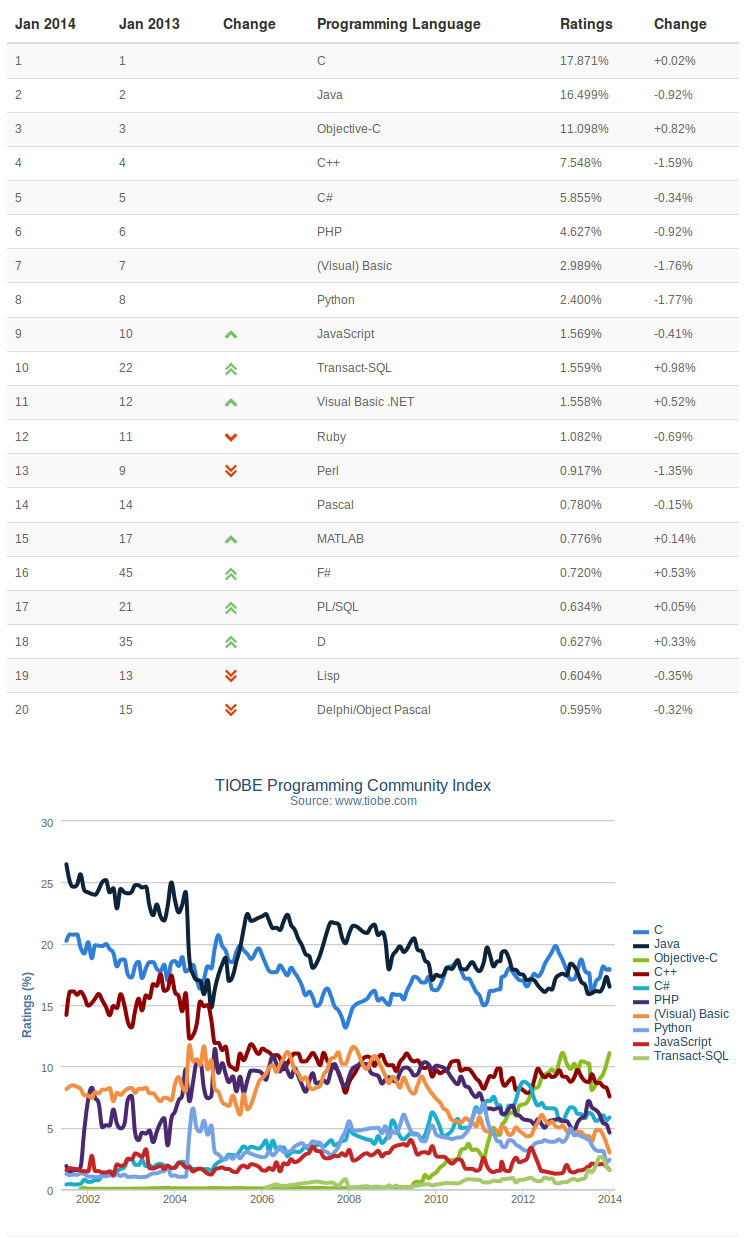
\includegraphics[height=564pt]{tiobe}
  \caption[Python popularity]{Popularity of Python compared to other
  languages\cite{website:tiobe-index}}
  \label{python-popularity}
\end{center}
\end{figure}

Python uses dynamic typing, also called duck typing. Duck typing doesn't check
if an object implements some certain interface, but simply tries to call the
method or attribute. The principle is ``If it looks like a duck and quacks like
a duck, it must be a duck''.\cite[duck-typing]{website:python-glossary} This
method of type checking renders interfaces useless. 

% XXX cite

% Python has two running modes: the interactive mode and the script mode. The
% interactive mode is a read-eval-print loop. It reads the user supplied
% \emph{expression} and parses it into a data structure, evaluates it and prints
% the result. An expression can't be multiline and must return only one value.
% Evaluating a value will return that value, evaluating a variable returns the
% contents of the variable and evaluating a function will call that function with
% the arguments and returns the result of the function. The script running mode is
% similar to the interactive mode, but instead of the user, the expressions are
% taken from a file and when the end of the file is reached, the interpreter
% terminates.

\subsubsection{Imperative programming}

Imperative programming is a style of programming with the philosophy of changing the machine's state to the required state, which could be a file in a hard drive or a video on the screen. For that the computer executes a sequence of operations in order, which are specified by the programmer. An operation is some change of state in the computer or calculation of some data.

\paragraph{Procedural programming}

Procedural programming is a subset of imperative programming. Procedural
programming tries to divide the program into variables, data structures and
procedures. Procedures are meant to group together abstract operations so they
could be reused in different situations. In this case an operation can also be a
procedure. Data structures are meant to group together conjoined data so they
could be moved and manipulated more easily. Variables are pointers to data. They
point to the location of the data in the memory which can be then easily
retrieved.

% XXX For now this fixes, that the below example isn't cut by the figure. Later,
% after everything above has been written, test if this is still necessary.

\clearpage

Python procedures look like this:
\begin{verbatim}
>>> def fib(n):    # write Fibonacci series up to n
...     """Print a Fibonacci series up to n."""
...     a, b = 0, 1
...     while a < n:
...         print a,
...         a, b = b, a+b
...
>>> # Now call the function we just defined:
... fib(2000)
0 1 1 2 3 5 8 13 21 34 55 89 144 233 377 610 987 1597
\end{verbatim}
\begin{quote}
``The keyword def introduces a function definition. It must be followed by the
function name and the parenthesized list of formal parameters. The statements
that form the body of the function start at the next line, and must be
indented.''\cite[4.6. Defining Functions]{website:python-functions}
\end{quote}
Python doesn't make a comparison between functions and procedures.

Each file in python is a module with the same name as the filename, except without the \texttt{.py} extension. Each module can import another module or every object in another modules namespace with the \texttt{import} command. When the import command is evaluated, the whole file is evaluated once. A directory can also be a module if it contains a \texttt{\_\_init\_\_.py} file. In that case the module is initialised with the \texttt{\_\_init\_\_.py} file and it's namespace contains the file modules in the directory.

% XXX Cite

% Procedures in Python are qcalled functions, because they can return one or
% multiple values, however if a return value isn't specified, it returns the
% \texttt{None} value. Python uses pass by reference so that values inside the
% object can be changed. However one must still be careful that changing the
% reference itself won't change the reference in the caller. Also even though
% numbers are objects and therefore are passed by reference, they are immutable
% and one can't change their inner value. That makes them in essence pass by
% value.

If a variable is nonlocal and the variable in the function is only read, then
the interpreter will try to find it from a nonlocal context. However, if the
variable is given new value anywhere in the function, the interpreter will
assume that the variable is local and the global variable will not be visible.
One can make a variable global with the \texttt{global} keyword. After that,
every reference to the variable will be a reference to the global variable.

\paragraph{Object-oriented programming}

Object-oriented programming is another subset of imperative programming.
Object-oriented programming tries to divide the program into objects that
communicate with each other. Each object has fields and methods. Fields and
methods are similar to variables and procedures, but they are tied to the
object. Fields are considered to be the objects inner state and methods are
considered to be the object's behaviour or object's
interface.\cite{website:object-orientation}

The goal of object-oriented programming is encapsulation. Encapsulation means
that each object has an inner state, inner behaviour and an interface for other
objects to use. An outer object doesn't need to know what is happening within
the object. It only needs to know how the object is going to react to an
interface procedure. Access protection modifiers are generally employed to
better enforce this behaviour. These modifiers are usually tied to a method or
field and they describe what other methods are allowed to access these methods
or fields. Right to access a field means the right to read or change the field
and right to access a method means the right to run the
method. An object's methods always have access to its objects
fields.\cite{website:access-modifiers}

An object can inherit another object. The inheriting object is called subobject and the inherited object is called the superobject. The subobject gets the superobject's fields and methods. A copy of the superobject is created and retained in the subobject. When searching for the subobject's methods or fields and they are not found then the superobject is searched for the field or method. A subobject doesn't automatically have access to the superobject's private fields and methods. The subobject can override the superobject's public methods. The type signature of the method cannot change, but the content or the action of the method is changed.

Class-based programming separates the object into the class and the instance.
The class is an abstraction and the classification of the object while the
instance is a actual object with actual data. Usually the class holds the
behaviour of the object, which includes the constructor. The constructor is a
special method, that is called when a new instance is being created from the
object. Inheritance works by remembering the inheritance line and then searching
for the methods in the right class.

An interface is a class that has no fields and all its methods are public. All
of the methods are abstract methods, meaning that the methods have no content or
implementation. A class can usually implement multiple interfaces but inherit
from only one class. One can't make a instance of an interface, there needs to
be an implementing class. An abstract class is a class that has atleast one
abstract method. Similar to interfaces, it is impossible to make an instance of
them. However they are still classes and and they are inherited, not
implemented.

Python has a class-based object-oriented style. Python, however, is more dynamic
than a normal static class-based language like Java. After an object has been
created from a class, one can still change that concrete object's variables and
methods. Every property is also public. Properties, that the programmer
considers private, are usually prefixed with underscores. Each statement is
evaluated top to bottom. If there are multiple properties with the same name,
then the last evaluated property is remembered.
\begin{verbatim}
class MyClass:
    """A simple example class"""
    i = 12345
    def f(self):
        return 'hello world'
\end{verbatim}

In Python, methods are functions, that get the object's instance in the first
parameter, but are called with the first parameter ignored, like this:
\verb;my_object.f();. If there are brackets after the class name and another
class's name inside the brackets, the class inherits from the class in the
bracket. A method can access the superclass with the \verb;super; function. The
super function takes two arguments: the type of the class of whose the super is
being searched for and the second is the object.

Multiple inheritance is supported by putting multiple class names in the
brackets supported by comas. If called for a property, that a object doesn't
have, the environment will try to find the property from the first named
superclass recursively until it hits object class and then the next superclass
recursively and so on. The object class is the superclass of every class. If
there are no brackets or the brackets are empty, then the object class is an
implicit superclass.

% XXX cite.

% Prototype-based programming is more used by dynamic languages. It keeps the
% design of the language minimal by having no wrappers around objects and their
% attributes. An object is created by creating an empty object or by cloning an
% existing object. Inheritance works by cloning an existing object and the subtype
% can replace the old attributes or add new attributes. Abstract objects are
% objects that will hold only behaviour by containing only constant or default
% attributes.


\subsubsection{Functional programming}

Functional programming languages are designed around functions. Programming
functions are similar to mathematical functions, that it has inputs as
parameters and returns a value as output. A function should always return the
same output with the same inputs and the inputs should not be changed inside the
function. This leads to a particularly stateless form of programming.

Due to the stateless form of this style, functional programming languages
usually support immutable datastuctures. Instead of updating a datastructure, it
is copied with the new values replaced and the new datastucture is returned.
First-class functions and dynamic evaluation of functions are also
supported.\cite{website:persistent-struct}

Python functions are very similar to Python procedures:
\begin{verbatim}
>>> def fib2(n): # return Fibonacci series up to n
...     """Return a list containing the Fibonacci series
...     up to n."""
...     result = []
...     a, b = 0, 1
...     while a < n:
...         result.append(a)    # see below
...         a, b = b, a+b
...     return result
...
>>> f100 = fib2(100)    # call it
>>> f100                # write the result
[0, 1, 1, 2, 3, 5, 8, 13, 21, 34, 55, 89]
\end{verbatim}
What has changed is that now the results are being collected into a list and
then the list is returned with the \verb;return;
keyword.\cite[4.6. Defining Functions]{website:python-functions}

A more functional way of programming would be this:
\begin{verbatim}
>>> def fib2(n): # return Fibonacci series up to n
...     """Return a list containing the Fibonacci series up to n."""
...     a, b = 0, 1
...     while a < n:
...         yield a    # see below
...         a, b = b, a+b
... 
>>> [a for a in fib2(100)]
[0, 1, 1, 2, 3, 5, 8, 13, 21, 34, 55, 89]
\end{verbatim}
In this example we don't change the list to collect the results, but instead
\verb;yield; the result. When the function is called, it will instead return a
generator. A generator is a simple data structure, that is iterable through
once and is only readable.
After a generator 

Generator is a data structure to dynamically iterate items. When a function has
a \texttt{yield} command somewhere inside of the function, when the function is
evaluated, the function is actually not run, but a generator data structure is
returned. The \texttt{yield} command is very similar to \texttt{return}, except
for one difference. When the generator is iterated, for example in a
\texttt{for} loop, the function is run until a \texttt{yield} command is hit,
the value is returned and the function is paused. When the next element is
requested, the function is continued again until the next \texttt{yield}. This
continues until the function reached the end, which signals that the generator
has no more elements. The advantage of a generator over a list for example, is
that lists require that all their elements are in memory at some point, while a generator has only one
element at a time in memory. Because when using a generator one can iterate over the items only once, there is also a slight speed increase. The disadvantages are that generators have no such data as the length of the iteration, are immutable and can't be iterated over for a second time.


\begin{quote}
``Small anonymous functions can be created with the \verb;lambda; keyword. This
function returns the sum of its two arguments: \verb;lambda a, b: a+b;. Lambda
functions can be used wherever function objects are required. They are syntactically restricted to a single expression. Semantically, they are just syntactic sugar for a normal function definition. Like nested function definitions, lambda functions can reference variables from the containing scope:''\cite[4.7.5. Lambda Expressions]{website:python-functions}
\end{quote}
\begin{verbatim}
>>> def make_incrementor(n):
...     return lambda x: x + n
...
>>> f = make_incrementor(42)
>>> f(0)
42
>>> f(1)
43
\end{verbatim}

Python has support fot lexical closures, which gives the function a strong
reference to the namespace. This excludes the possibility that the namespace will be garbage
collected while the function is still in memory. The function has the guarantee
that the non-local values will exist even after the enclosing context is deleted
or garbage collected.\cite{website:python-closures}

Since other functional languages have them, Python also has functions
\verb;map;, \verb;filter; and \verb;reduce;. \verb;map; applies a function
to every item in an iterable and returns a new list with the results of the
function. \verb;filter; applies a function to every item in an iterable and
returns a new list with the items where the function returned \verb;True;. And \verb;reduce; applies a function for every item in an iterable and returns the value of the last evaluation. In this case the function must have two parameters and the first parameter holds the value from the last evaluation of the function.

A way to avoid using \verb;map; and \verb;filter; is by generator expressions
and list comprehensions. List comprehensions are a syntactic sugar to easily
create lists. Unlike \verb;map;, list comprehensions don't need to be supplied a
function, but can also use arbitrary expressions. A sample list comprehension
is: \verb;[2 * item for item in iterable if item % 2 == 0];. This expression
returns a filtered list where each element of iterable is multiplied with 2. The
returned list contains only elements that were even before. Therefore the syntax
is
\verb;[expression for expr1 in sequence1 if condition1 for expr2 in sequence2 if condition2 ...];.
The commands are nested with the right being inside the left and the first expression being the returned innermost expression. Generator expressions are syntactically same, except normal brackets instead of square brackets are used and they create a generator instead of a
list.

\subsubsection{Implementation}

A programming language by itself is not useful. It also needs an implementation.
An implementation is a program that evaluates the syntax of the program into
machine actions. There are 3 ways to create an implementation:
\begin{description}
  \item[Interpretation] Interpretation parses the source code and performs the
  instructions directly
  \item[Compilation] Compilation is transforming the current source code into a
  another format that can then be interpreted. Compiled language can also
  compile into another compiled language which will compile that into another
  language and so on.
  \item[just-in-time (JIT) compilation] JIT takes a hybrid approach of
  interpretation and compilation. While interpreting the program, the JIT
  compiler will observe what parts of the program are most often interpreted and
  will compile those parts.
\end{description}
Generally the compiling phase is called the compile time and the interpretation
phase is called the runtime. Compiled languages are usually considered fastest,
because compilation can heavily optimise the programmer's code, which leads to
a faster runtime. Interpretation however is faster and easier to use for the
programmer because the compilation step is skipped. For this reason interpreted
languages are usually used for scripting. JIT implementations are usually as easy to use as interpreted implementations, but
are a lot faster. However because the analysation is fairly complex and runs
parallel to the execution of the program, JIT compilers take a lot more
memory.\cite{website:jit-memory}

The official implementation of Python is CPython. Every formal change to the
language will be almost immediately mirrored in this implementation. It will be
supported for a long time will be the most current and up-to-date compared to
other implementations. CPython is a bytecode interpreter. It compiles to an
intermediate bytecode, which it then interprets. It compiles every time the
source file has been changed. This implementation is slow compared to
other languages\cite{website:python-speed}, but enables hooking the script to a
C module. Since the C programming language is fast,\cite{website:c-vs-python} it
is possible to write most of the program in Python and write the bottlenecks in
C.

The most popular alternative implementation to CPython is \pypy. \pypy{} is a JIT
compiler written in Python. It is popular because of its speed. As of \today,
\pypy{} is about 6.2~times faster than pure
CPython.\cite{website:python-pypy-speed} There are two disadvantages: \pypy{}
doesn't have hooks into C and PyPy isn't as up-to-date as CPython. As of \today,
Python 3 support for \pypy is in the beta state while CPython supports Python
3.4.0. Also since PyPy doesn't have hooks into C, it can't speed up the
bottlenecks of a program. With simple calculation from
\cite{website:c-vs-python,website:python-pypy-speed}, C gcc is still about 3
times faster than PyPy.

There are also Jython and IronPython. Jython compiles down to Java bytecode. It
allows the programmer to use libraries from Java in his project. IronPython is
the same principle, only it compiles to the .NET bytecode. That gives IronPython
projects access to .NET libraries.
